\begin{frame}{Quittons la ville!}
  \begin{columns}
    \column{0.5\textwidth}
      \begin{center}
        \small
        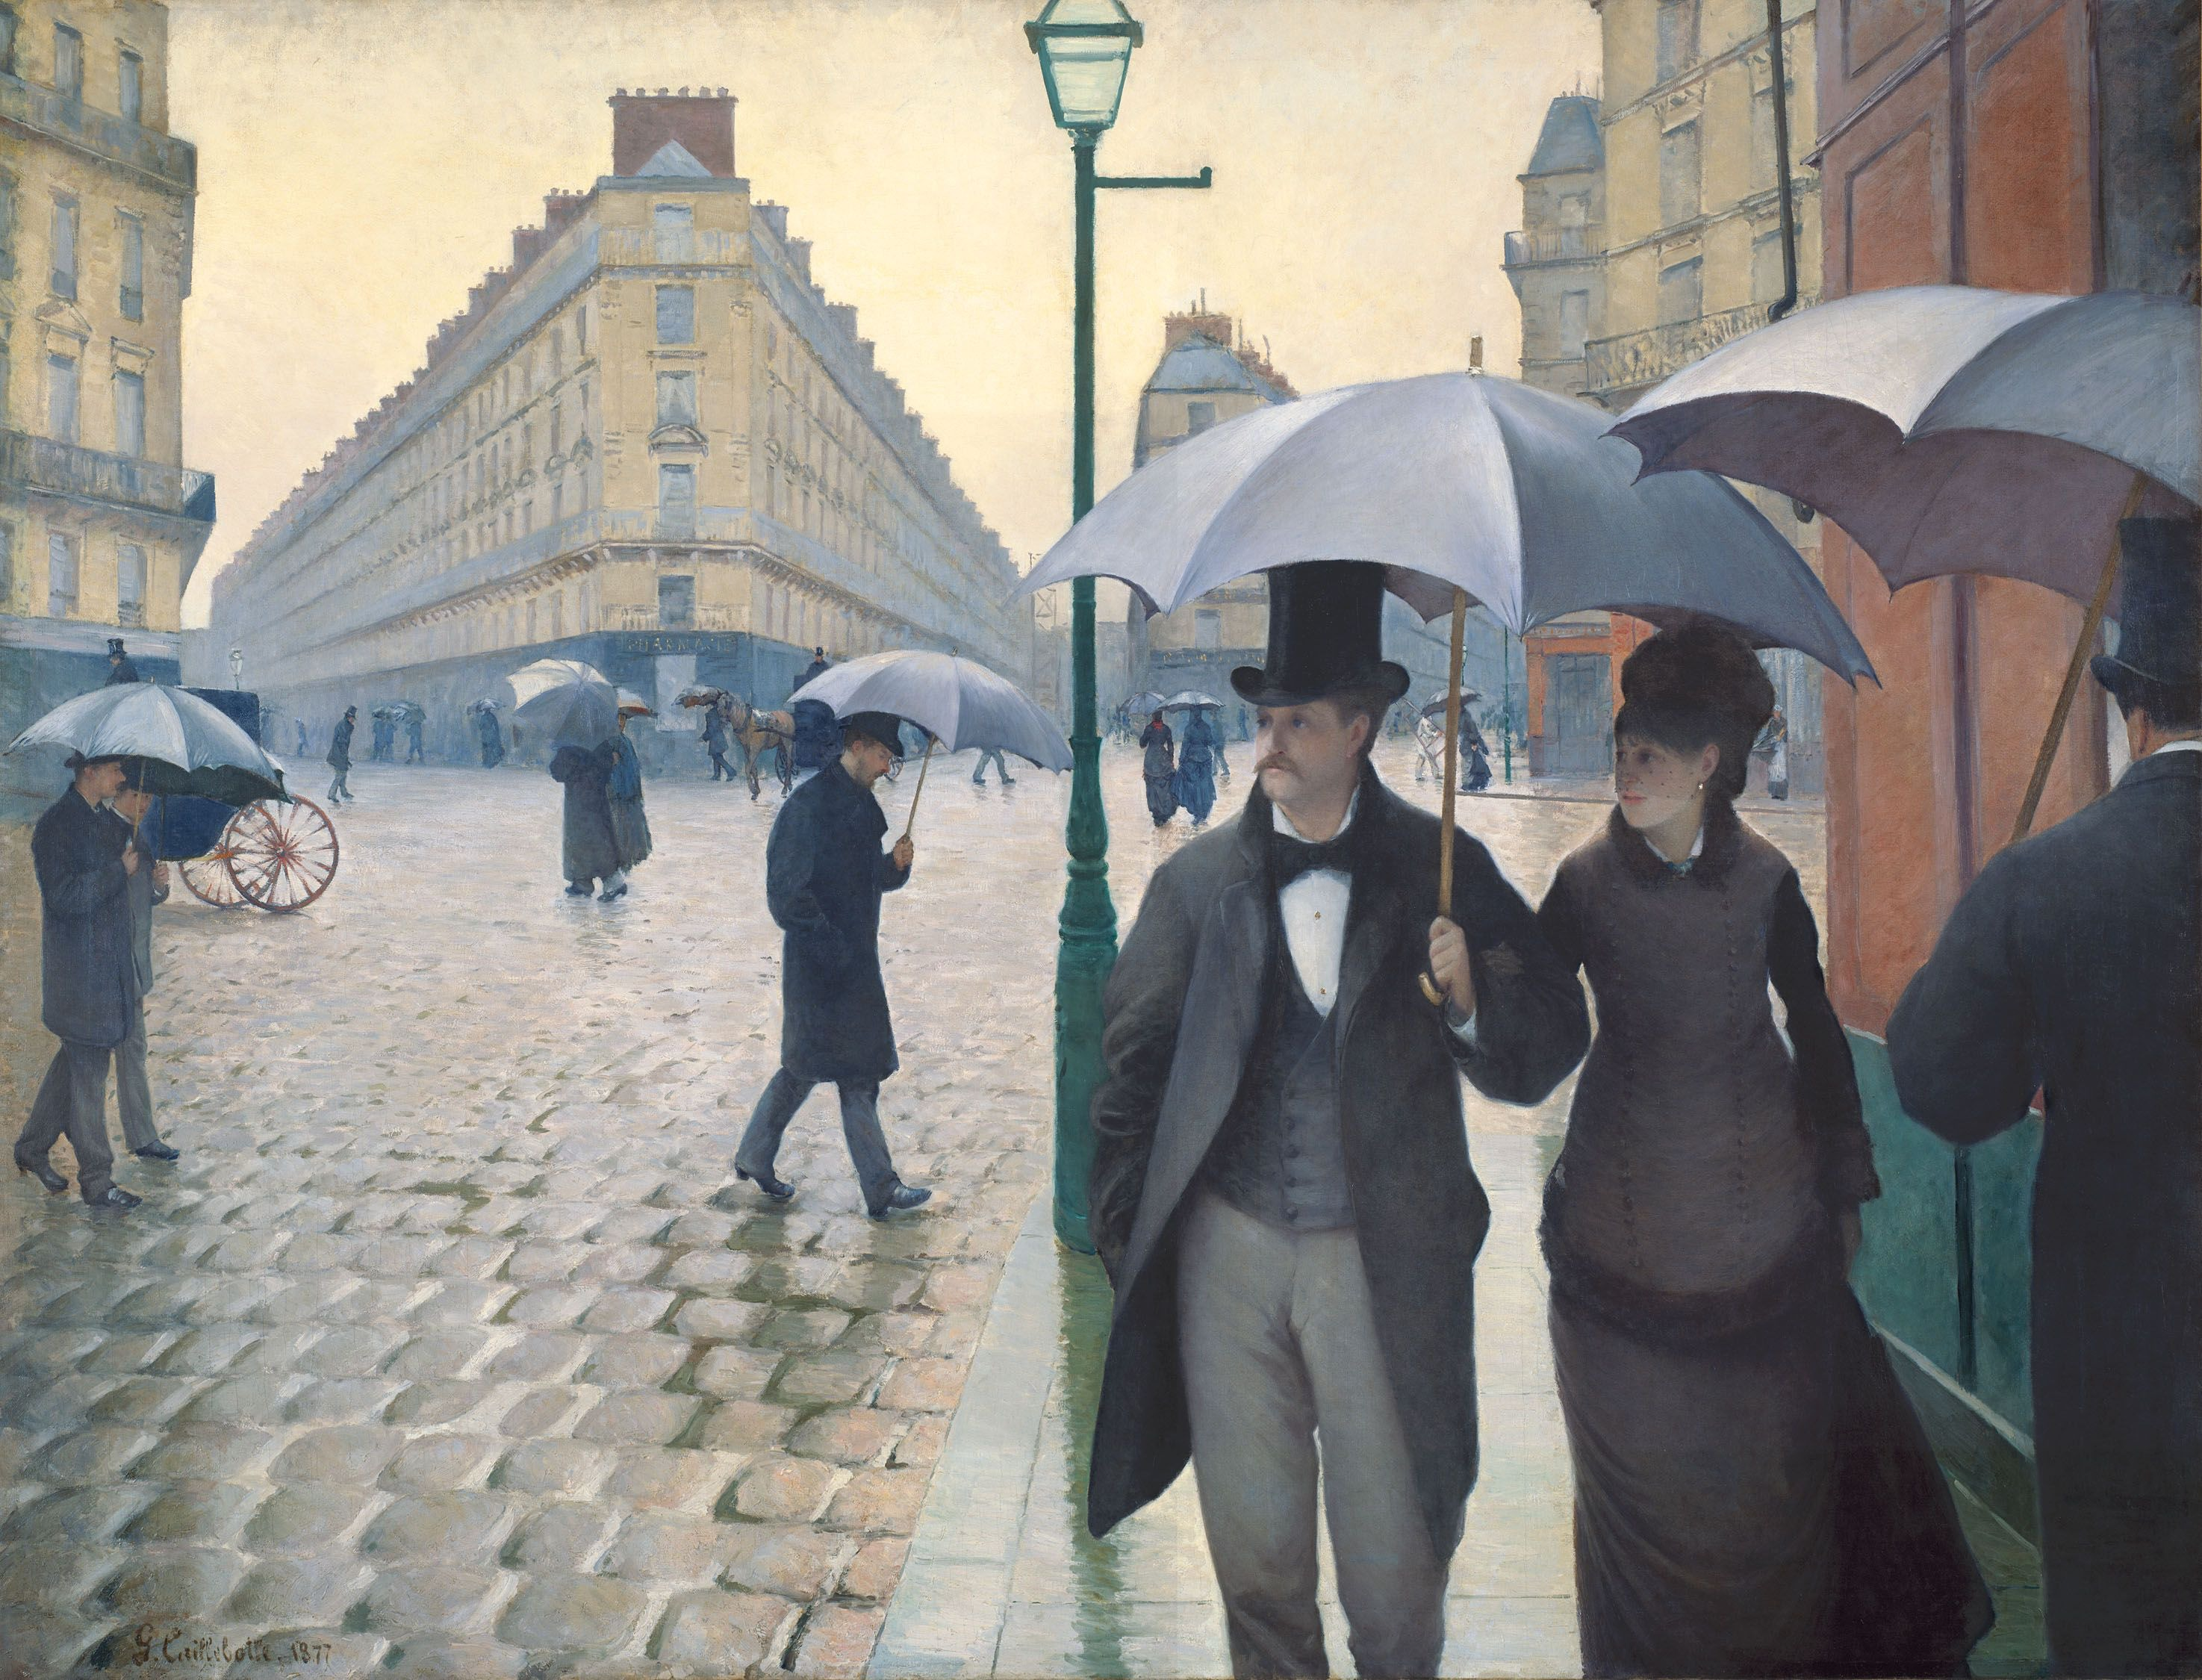
\includegraphics[scale=0.05]{gustave_caillebotte.jpg} \\
        Gustave Caillebotte (1848-1894) \\
        \emph{Rue de Paris, temps de pluie}, 1877
      \end{center}
    \column{0.5\textwidth}
      Écoutons ensemble les plaintes d'Amélie concernant la vie à Paris.
      Dans chaque phrase, il y a un adverbe.
      Écris l'adjectif qui y correspond sur un papier.
      \begin{itemize}
        \item \textbf{Modèle:}
        \item Elle dit: \emph{La vie à Paris est horriblement chère.}
        \item Tu écris: horrible
      \end{itemize}
  \end{columns}
\end{frame}